\subsection{Loop ordering}\label{sec:loopordering}
One of the optimizations we attempted was to change the ordering of the loops.
With a blocked strategy, there are two different places where the loop ordering
can be changed: Changing the order in which the blocks are processed, and
changing the loop ordering inside of each block multiplication.

\subsubsection{Inside loop ordering}
When multiplying the blocks, we see that there are three index variables:
$i,j,$ and $k$. Changing the ordering of these loops affects the stride and
regularity at which we access memory, which can have a significant effect upon
performance.

We note that there are $3! = 6$ possible orderings of these loops. In order to
determine which was fastest, we tested and compared all 6 on the totient node.
Note that we kept the outside loop ordering constant for all of these, as we
assumed that the inside and outside loop orderings were orthogonal, or at least
close enough that the difference was not significant. The results can be found
in the following figure:

\begin{figure}[hh]
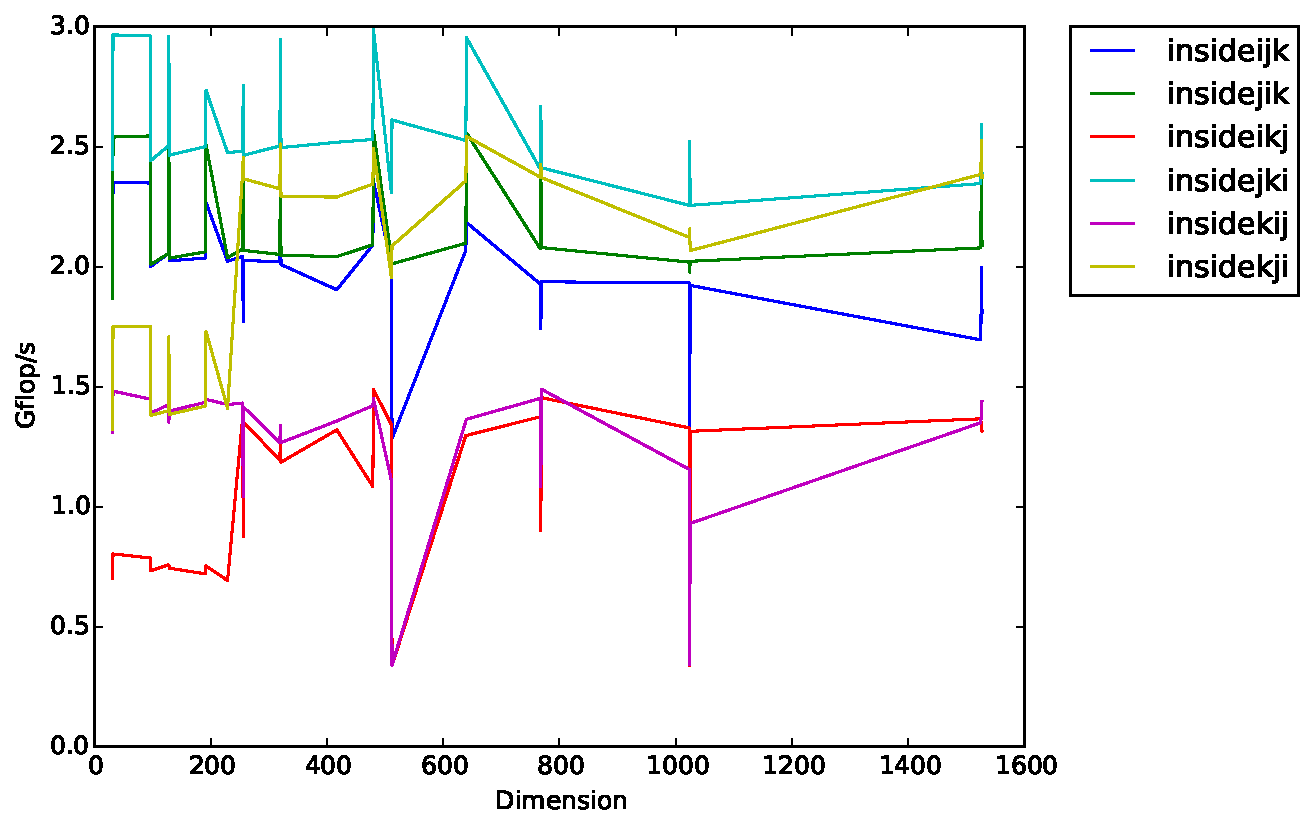
\includegraphics[width=0.75\textwidth]{timing_insideloops.pdf}
\caption{Timing results for the different inside loop orderings}
\end{figure}
Here we see that the loop ordering of $j,k,i$ was clearly fastest, and
significantly faster than the slowest loop orderings.

\newpage
\subsubsection{Outside loop ordering}
Similarly, the order in which we choose which blocks to multiply can also be
changed around. Again, we compared the six different possible orderings, while
keeping the inside loop ordering fixed as $j,k,i$, which was found to be the
fastest in the previous subsection. The timing results are found in the
following figure:

\begin{figure}[hh]
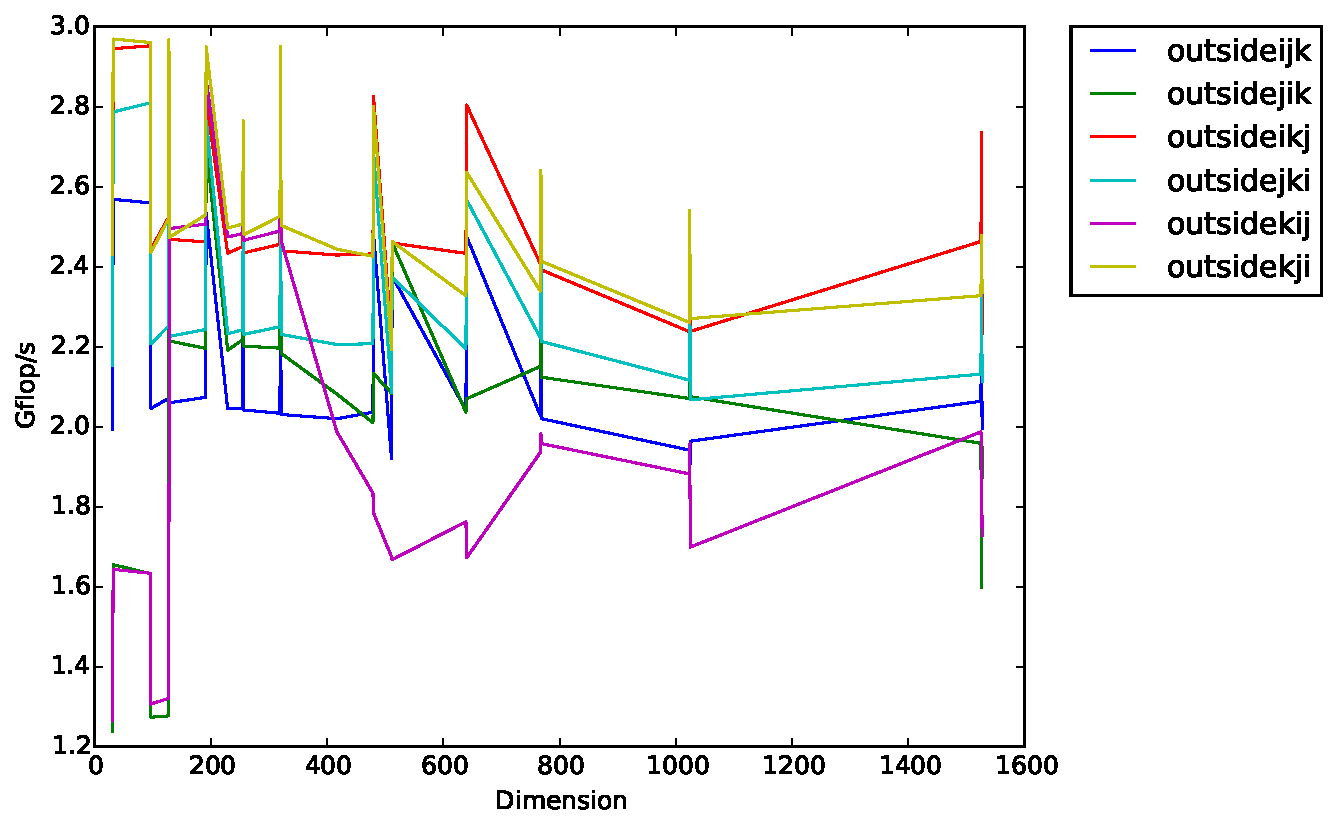
\includegraphics[width=0.75\textwidth]{timing_outsideloops.pdf}
\caption{Timing results for the different outside loop orderings}
\end{figure}

Here we see that some loop orderings are definitely faster than others, but
this time there is no clear best ordering as both $k,j,i$ and $i,k,j$ are
fastest on different size matrices. We chose to go with the outside loop
ordering $i,k,j$

Unfortunately, our results for loop ordering are mostly incompatible with the
work done on copy optimization, as certain inside loop orderings are faster
because of the stride of the data access, but copy optimization changes this so
that data is generally accessed at unit stride.
